% !TeX root = ../../Book3.tex
\chapter{算术函数与 Dirichlet 级数}
\label{b3:ch:25}
\BookChapterNumber{b3:ch:25}

\begin{chapterabstract}
整数的唯一素分解怎样进入复分析？本章先从有限的约数求和出发，建立可乘函数、Dirichlet 卷积和 Möbius 反演；再用 Abel 求和保留系数部分和的抵消，说明 Dirichlet 级数的收敛半平面、乘法、求导与求逆。在明确的绝对收敛域内，Euler 乘积把整数系数分解为素数幂因子，它的对数与对数导数进一步产生素数权重。除数平均、平方自由密度及互素整数对计数将说明这些转换如何得到可检验的算术结论。
\end{chapterabstract}

\begin{learninggoals}
能够从素数幂值计算可乘函数，区别逐点乘法与 Dirichlet 卷积，并用递推逆元和 Möbius 反演恢复系数；能够完整写出部分求和的端点项，依据部分和增长估计加权尾和；能够区分普通收敛、绝对收敛与解析延拓，检查无穷乘法及取商的条件；能够由 Euler 乘积构造全纯对数，解释 von Mangoldt 权重的来源，并估计算术计数中的取整误差。
\end{learninggoals}

上一编已经遇到一些由整数决定的系数：Eisenstein 级数的展开含有约数幂和 \(\sigma_3(n),\sigma_5(n)\)，theta 级数的系数则计数平方和表示。它们看起来属于不同问题，却都受到整数乘法结构的制约。比如，把一个整数写成互素因子的乘积，往往可以将它的约数或表示数分成两部分计算。本章把这些共同的操作单独整理出来。

复分析中的变量是连续的，素数却形成离散且不规则的集合。为了连接两者，给每个正整数指定权重 \(a(n)\)，再考虑
\[
 \sum_{n\ge1}\frac{a(n)}{n^s},\qquad s=\sigma+\mathrm it.
\]
增大 \(\sigma\) 会压低大整数的贡献；改变 \(t\) 则通过 \(e^{-\mathrm it\log n}\) 改变相位。这个构造有很强的表达能力，但不能只把一个形式公式写成级数就认为它已定义解析函数：系数如何增长、是否相消、求和次序能否改变，都需要具体判断。

本章按这些问题出现的顺序展开。前两节只做有限算术运算，约数卷积和反演在这里不需要收敛条件。第三节利用部分和 \(A(x)=\sum_{n\le x}a(n)\) 处理加权和，并通过双曲线计数求出除数函数的平均值。第四节建立级数的半平面理论，说明有限卷积在什么条件下对应函数乘法及倒数。第五节再把可乘性变成 Euler 乘积，用收敛对数排除零点，推导 \(-\zeta'/\zeta\) 的素数幂系数。

Apostol 的《Introduction to Analytic Number Theory》\cite{Apostol1976Introduction}可作为算术函数、部分求和及初等解析数论的进一步读物。阅读具体级数时，可先问系数的部分和有多大，再比较逐项取绝对值以后损失了多少抵消；这两种估计将给出不同的收敛范围。

% !TeX root = ../../Book3.tex
\section{算术函数}
\label{b3:sec:2501}

前两章出现的 \(\sigma_3(n)\)、\(\sigma_5(n)\) 和平方和表示数，都是以正整数为自变量的函数。它们的数值并非彼此孤立：一个整数怎样分解成素数，往往决定相应系数怎样计算。本章先整理这种有限的分解结构，再把系数放入复变级数。这样安排可以分清两类问题：一个恒等式是否在每个整数处成立，以及把这些恒等式无限相加是否合法。

以下约数均指正约数，素数均指正素数。若 \(p\) 为素数，记 \(p^r\parallel n\) 表示 \(p^r\mid n\) 而 \(p^{r+1}\nmid n\)。在乘积 \(\prod_{p^r\parallel n}\) 中只取 \(r\ge1\)；\(n=1\) 时乘积为空，约定值为 \(1\)。算术基本定理说，每个 \(n>1\) 都唯一写成
\[
 n=p_1^{r_1}\cdots p_\ell^{r_\ell},
 \qquad p_1<\cdots<p_\ell,\quad r_j\ge1.
\]
这里每个整数只涉及有限多个素数。即使我们同时给所有素数规定参数，计算一个固定整数处的值仍然只做有限次运算；这一点与后面真正的无穷 Euler 乘积不同。

\subsection{可乘函数}
\label{b3:subsec:250101}

如果 \(m,n\) 互素，它们的素因子集合没有交叠，因而 \(mn\) 的分解只是把两组素数幂放在一起。这提示我们先研究能够随这种分解而分离的函数。

\begin{definition}\label{b3:def:25-multiplicative}
从正整数集合 \(\mathbb N_{\ge1}\) 到 \(\mathbb C\) 的函数称为\term[suanshu-hanshu]{算术函数}[arithmetic function]。若算术函数 \(a\) 满足 \(a(1)=1\)，并且对任意互素的正整数 \(m,n\) 有
\[
 a(mn)=a(m)a(n),
\]
则称 \(a\) 为\term[kecheng-hanshu]{可乘函数}[multiplicative function]。
\end{definition}

定义只对互素输入提出乘法要求，因此不能未经说明便把 \(a(p^2)\) 写成 \(a(p)^2\)。实际上，所有素数幂处的值都是独立的初始数据。

\begin{proposition}[素数幂决定可乘函数]
\label{b3:prop:25-prime-power-data}
若 \(a:\mathbb N_{\ge1}\to\mathbb C\) 可乘，则对每个正整数 \(n\) 有
\[
 a(n)=\prod_{p^r\parallel n}a(p^r).
\]
反之，对每个素数 \(p\) 和整数 \(r\ge1\) 任意指定一个复数 \(c_{p,r}\)，并令
\[
 a(1)=1,\qquad
 a(n)=\prod_{p^r\parallel n}c_{p,r}\quad(n>1),
\]
便得到唯一满足 \(a(p^r)=c_{p,r}\) 的可乘函数；不需要对这些复数作有界性或非零性假设。
\end{proposition}
\begin{proof}
同一整数的不同素数幂因子两两互素。反复使用定义，便得到第一个公式。反过来，素因子分解的唯一性保证所给公式没有选择上的歧义；每个乘积有限，保证其值是一个确定的复数。若 \(m,n\) 互素，二者的素因子集合不交，所以定义 \(a(mn)\) 的有限乘积恰能拆成定义 \(a(m)\) 和 \(a(n)\) 的两个乘积。这证明可乘性，也证明了唯一性。
\end{proof}

例如 \(72=2^3\cdot3^2\)，所以可乘性给出 \(a(72)=a(8)a(9)\)，却没有给出 \(a(8)\) 与 \(a(2)\) 的关系。即使 \(a(2)=0\)，一般的可乘函数仍可以满足 \(a(4)=1\)。在后面的 Euler 因子中，必须把 \(a(p),a(p^2),\ldots\) 全部保留下来，原因就在这里。

定义中的 \(a(1)=1\) 也不是无关紧要的附注。假如只要求互素时的乘法公式，把 \(m=1\) 代入就有 \(a(n)=a(1)a(n)\)。若函数至少在一处非零，这个等式强制 \(a(1)=1\)；否则零函数也会满足该公式。本书把零函数排除在可乘函数之外，使所有可乘函数都具有相同的单位规范化。

\subsection{完全可乘函数}
\label{b3:subsec:250102}

互素的限制一旦去掉，同一个素数的重复出现也必须服从乘法规则。这比上一小节的要求强得多。

\begin{definition}\label{b3:def:25-completely-multiplicative}
若算术函数 \(a:\mathbb N_{\ge1}\to\mathbb C\) 满足 \(a(1)=1\)，并且对任意正整数 \(m,n\) 都有 \(a(mn)=a(m)a(n)\)，则称 \(a\) 为\term[wanquan-kecheng-hanshu]{完全可乘函数}[completely multiplicative function]。
\end{definition}

\begin{proposition}[完全可乘性的素数判据]
\label{b3:prop:25-completely-prime-data}
算术函数 \(a:\mathbb N_{\ge1}\to\mathbb C\) 完全可乘，当且仅当它可乘，且对每个素数 \(p\) 与每个整数 \(r\ge1\) 都有 \(a(p^r)=a(p)^r\)。因此，任意指定复数 \(c_p\) 后，公式
\[
 a(1)=1,\qquad a(n)=\prod_{p^r\parallel n}c_p^r
\]
给出唯一满足 \(a(p)=c_p\) 的完全可乘函数。
\end{proposition}
\begin{proof}
完全可乘时，逐次把 \(p^r\) 分成 \(p^{r-1}p\)，便得所列幂次关系。反过来，设各素数在 \(m,n\) 中的指数分别为 \(u_p,v_p\)，允许其中之一为零。只在 \(mn\) 的有限个素因子上取乘积，就有
\[
 a(mn)=\prod_{p\mid mn}a(p)^{u_p+v_p}
       =\left(\prod_{p\mid mn}a(p)^{u_p}\right)
        \left(\prod_{p\mid mn}a(p)^{v_p}\right)
       =a(m)a(n).
\]
指数为零的因子按空乘积理解为 \(1\)，所以即使某个 \(a(p)=0\)，该论证也适用。
\end{proof}

对任意固定的 \(\alpha\in\mathbb C\)，函数 \(n\mapsto n^\alpha\) 完全可乘，其中
\[
 n^\alpha=\exp(\alpha\log n)
\]
使用正实数的实对数。这里 \(\log(mn)=\log m+\log n\)，没有复对数的分支问题。另一方面，记 \(d(n)\) 为 \(n\) 的正约数个数，则 \(d(p)=2\)、\(d(p^2)=3\)，所以 \(d(p^2)\ne d(p)^2\)。稍后会证明 \(d\) 可乘，但这个简单计算已说明它不完全可乘。

完全可乘函数仍然允许零值。例如，固定素数 \(p_0\)，令 \(a(n)=0\) 当 \(p_0\mid n\)，否则令 \(a(n)=1\)，就得到完全可乘函数。一般地，若 \(a(p_0)=0\)，每个含 \(p_0\) 的整数都必须取值零。这比仅有可乘性时的结论更强；后面模整数的特征标也会出现这种零值。

\subsection{Möbius 函数 \texorpdfstring{\(\mu\)}{\AnalysisPdfMu}}
\label{b3:subsec:250103}

容斥原理用交替的正负号消去重复计数。若需要同时排除若干素数的整除性，选择一个素数子集就相当于选择这些素数的乘积。Möbius 函数把这个子集符号写成一个算术函数。

\begin{definition}\label{b3:def:25-mobius}
正整数 \(n\) 称为\term[pingfang-ziyou-zhengshu]{平方自由整数}[squarefree integer]，如果没有素数 \(p\) 满足 \(p^2\mid n\)。在正整数上定义\term[mobius-hanshu]{Möbius 函数}[Möbius function]
\[
 \mu(n)=
 \begin{cases}
  1,&n=1,\\
  (-1)^r,&n=p_1\cdots p_r,\quad p_1,\ldots,p_r\text{ 为互异素数},\\
  0,&n\text{ 不是平方自由整数}.
 \end{cases}
\]
\end{definition}

因此 \(\mu(p)=-1\)，而 \(\mu(p^r)=0\) 对 \(r\ge2\) 成立。互素相乘时，如果任一因子含有平方素因子，乘积也含有；如果两因子都平方自由，乘积的不同素因子数就是二者的和。这分别证明了两种情形下的 \(\mu(mn)=\mu(m)\mu(n)\)，故 \(\mu\) 可乘。它不完全可乘，因为 \(\mu(p^2)=0\ne1=\mu(p)^2\)。

\begin{proposition}\label{b3:prop:25-mobius-sum}
设 \(\mu\) 为 Möbius 函数，\(n\ge1\) 为整数。则
\[
 \sum_{d\mid n}\mu(d)=
 \begin{cases}1,&n=1,\\0,&n>1.\end{cases}
\]
\end{proposition}
\begin{proof}
设 \(n\) 的不同素因子为 \(p_1,\ldots,p_r\)。和中的非零项恰好对应这些素数的子集：选取子集 \(J\) 后，相关约数为 \(\prod_{j\in J}p_j\)，符号为 \((-1)^{|J|}\)。所以当 \(n>1\) 时，\(r\ge1\)，并且
\[
 \sum_{d\mid n}\mu(d)
 =\sum_{J\subseteq\{1,\ldots,r\}}(-1)^{|J|}
 =\sum_{j=0}^r\binom rj(-1)^j=(1-1)^r=0.
\]
当 \(n=1\) 时只有约数 \(1\)，和就是 \(\mu(1)=1\)；也可以把它理解为不含任何因子的空乘积。
\end{proof}

例如 \(12\) 的约数中只有 \(1,2,3,6\) 提供非零项，因而该和为 \(1-1-1+1=0\)。虽然 \(12\) 含有 \(2^2\)，容斥只关心素数 \(2\) 是否被选中；重复选择同一个排除条件不会产生新的交集。下一节正是利用这个消去恒等式，把已经做过的约数求和逆转回来。

\subsection{Euler 函数 \texorpdfstring{\(\varphi\)}{\AnalysisPdfVarPhi}}
\label{b3:subsec:250104}

一个具体的计数问题是：在 \(1,\ldots,n\) 中，有多少整数没有与 \(n\) 共有的素因子？这也就是模 \(n\) 的可逆剩余类的个数，不过当前只需要互素计数这一解释。

\begin{definition}\label{b3:def:25-totient}
对每个正整数 \(n\)，定义\term[euler-hanshu]{Euler 函数}[Euler totient function]
\[
 \varphi(n)=\#\{a\in\mathbb Z:1\le a\le n,\ \gcd(a,n)=1\}.
\]
特别地，\(\varphi(1)=1\)。
\end{definition}

\begin{proposition}[Euler 函数的两个计数公式]
\label{b3:prop:25-totient-identities}
对每个正整数 \(n\)，有
\[
 \varphi(n)=n\prod_{p\mid n}\left(1-\frac1p\right),
 \qquad
 \sum_{d\mid n}\varphi(d)=n.
\]
其中第一式在 \(n=1\) 时采用空乘积约定。函数 \(\varphi\) 可乘，且对素数 \(p\) 和整数 \(r\ge1\) 有 \(\varphi(p^r)=p^r-p^{r-1}\)。
\end{proposition}
\begin{proof}
设 \(p_1,\ldots,p_\ell\) 是 \(n>1\) 的不同素因子。不与 \(n\) 互素的整数，正是至少被一个 \(p_j\) 整除的整数。对这些整除条件应用有限容斥：若选取素数子集 \(J\)，同时被其中所有素数整除的整数共有
\[
 \frac{n}{\prod_{j\in J}p_j}
\]
个。这里不需要取整，因为分母整除 \(n\)。于是
\[
 \varphi(n)
 =n\sum_{J\subseteq\{1,\ldots,\ell\}}
     \frac{(-1)^{|J|}}{\prod_{j\in J}p_j}
 =n\prod_{j=1}^{\ell}\left(1-\frac1{p_j}\right).
\]
当 \(n=1\) 时公式由定义成立。互素的 \(m,n\) 具有不相交的素因子集合，第一式因而给出 \(\varphi(mn)=\varphi(m)\varphi(n)\)；代入 \(n=p^r\) 就得到素数幂公式。

为证明第二式，把 \(1,\ldots,n\) 按 \(\gcd(a,n)=d\) 分组。只有 \(d\mid n\) 的组可能非空。写成 \(a=db\) 后，该组与
\[
 1\le b\le n/d,\qquad \gcd(b,n/d)=1
\]
的整数一一对应，所以该组有 \(\varphi(n/d)\) 个元素。各组不相交且合起来有 \(n\) 个元素，故 \(n=\sum_{d\mid n}\varphi(n/d)\)。再把约数 \(d\) 换成 \(n/d\)，即得第二式。
\end{proof}

例如，当 \(n=12\) 时，要从十二个整数中减去六个偶数和四个 \(3\) 的倍数，再加回被减了两次的两个 \(6\) 的倍数，因此 \(\varphi(12)=12-6-4+2=4\)。余下的整数为 \(1,5,7,11\)。这个例子也解释了乘积中的 \(1-1/p\)：它记录排除一个素数整除条件所产生的比例；不同素数之间的交集由容斥精确处理，不能仅凭未经证明的“独立性”猜出乘积。

\subsection{除数函数}
\label{b3:subsec:250105}

平方和公式和 Eisenstein 级数的 Fourier 展开把许多系数写成约数的幂次和。统一记号之后，约数个数、约数总和以及复参数加权就可以一同处理。

\begin{definition}\label{b3:def:25-divisor-functions}
设 \(\alpha\in\mathbb C\)。对每个正整数 \(n\)，定义\term[chushu-hanshu]{除数函数}[divisor function]
\[
 \sigma_\alpha(n)=\sum_{d\mid n}d^\alpha,
 \qquad d^\alpha=\exp(\alpha\log d),
\]
其中 \(\log d\) 为实对数。记 \(d(n)=\sigma_0(n)\)，即 \(n\) 的正约数个数；\(\sigma_1(n)\) 是其正约数之和。
\end{definition}

\begin{proposition}[除数函数的局部公式]
\label{b3:prop:25-divisor-local}
对每个固定的 \(\alpha\in\mathbb C\)，函数 \(\sigma_\alpha\) 可乘。对素数 \(p\) 与整数 \(r\ge0\)，有
\[
 \sigma_\alpha(p^r)=\sum_{j=0}^r p^{j\alpha}
 =\begin{cases}
 \displaystyle\frac{p^{(r+1)\alpha}-1}{p^\alpha-1},&p^\alpha\ne1,\\[6pt]
 r+1,&p^\alpha=1.
 \end{cases}
\]
特别地，\(d(n)=\prod_{p^r\parallel n}(r+1)\)。
\end{proposition}
\begin{proof}
当 \(m,n\) 互素时，\(mn\) 的每个约数唯一写成 \(uv\)，其中 \(u\mid m\)、\(v\mid n\)：把约数中的素数幂分别分配给 \(m\) 和 \(n\) 即得。利用 \((uv)^\alpha=u^\alpha v^\alpha\)，便有
\[
 \sigma_\alpha(mn)
 =\sum_{u\mid m}\sum_{v\mid n}u^\alpha v^\alpha
 =\sigma_\alpha(m)\sigma_\alpha(n).
\]
素数幂 \(p^r\) 的约数恰为 \(1,p,\ldots,p^r\)，所以局部公式是有限几何和。若公比 \(p^\alpha\ne1\)，将这个和乘以 \(p^\alpha-1\) 得到分式；若公比为 \(1\)，则每一项都是 \(1\)，共有 \(r+1\) 项。令 \(\alpha=0\) 并使用可乘性，得到最后一个公式。
\end{proof}

复参数时，分母为零的例外不只发生在 \(\alpha=0\)。对固定素数 \(p\)，准确条件是
\[
 p^\alpha=1
 \quad\Longleftrightarrow\quad
 \alpha\log p\in2\pi i\mathbb Z.
\]
例如 \(\alpha=2\pi i/\log2\) 时，\(\sigma_\alpha(2^r)=r+1\)。因此应当先使用有限和定义，再判断某个几何和分式能否代入。每个固定 \(n\) 的 \(\sigma_\alpha(n)\) 本来就是关于 \(\alpha\) 的有限指数和，并没有真正的奇点。

对 \(12=2^2\cdot3\)，局部计算给出
\[
 d(12)=(2+1)(1+1)=6,
 \qquad \sigma_1(12)=(1+2+4)(1+3)=28.
\]
这个计算免去了逐个列出约数；前两章的 \(\sigma_3\)、\(\sigma_5\) 也服从同样的素数幂分解。

为了把这些系数放进级数，需要先知道它们不会增长得过快。粗略地说，\(d(n)\le n\) 当然成立，但这个界会把可保证收敛的半平面推得过于靠右。下面的估计利用素数幂结构，把增长压到任意指定的正幂以下。

\begin{proposition}[除数个数的缓慢增长]
\label{b3:prop:25-divisor-small-power}
令 \(d(n)\) 为正整数 \(n\) 的正约数个数。对每个实数 \(\varepsilon>0\)，存在只依赖于 \(\varepsilon\) 的常数 \(C_\varepsilon>0\)，使所有正整数满足
\[
 d(n)\le C_\varepsilon n^\varepsilon.
\]
\end{proposition}
\begin{proof}
要估计乘积 \(d(n)=\prod_{p^r\parallel n}(r+1)\)，希望把每个因子 \(r+1\) 吸收到 \(p^{r\varepsilon}\) 中。若 \(p^\varepsilon\ge2\)，则对 \(r\ge1\) 有
\[
 r+1\le2^r\le p^{r\varepsilon};
\]
其中第一步可由二项式展开 \(2^r=(1+1)^r\ge1+r\) 得到。这些较大的素数不需要额外常数。

剩下的素数满足 \(p<2^{1/\varepsilon}\)，所以只有有限个。对每个这样的 \(p\)，数列 \((r+1)p^{-r\varepsilon}\) 有有限上界：相邻两项之比为
\[
 \frac{r+2}{r+1}p^{-\varepsilon}\longrightarrow p^{-\varepsilon}<1,
\]
因而从某一项起几何衰减。令
\[
 C_{p,\varepsilon}=\sup_{r\ge0}(r+1)p^{-r\varepsilon},
 \qquad
 C_\varepsilon=\prod_{p<2^{1/\varepsilon}}C_{p,\varepsilon}.
\]
每个局部常数至少为 \(1\)，总乘积有限。对 \(n\) 的每个素数幂使用上述相应估计，再把没有出现在 \(n\) 中的小素数因子补进常数，就有
\[
 d(n)\le C_\varepsilon\prod_{p^r\parallel n}p^{r\varepsilon}
       =C_\varepsilon n^\varepsilon.
\]
\end{proof}

这里必须先固定 \(\varepsilon\)，再选择常数。不能令 \(\varepsilon\downarrow0\) 而保持同一个 \(C_\varepsilon\)，进而宣称 \(d(n)\) 有界。例如，若 \(n\) 是 \(k\) 个不同素数的乘积，则 \(d(n)=2^k\)。该命题比较的是增长阶，并未给出一个与 \(\varepsilon\) 无关的统一上界。

对复参数也能直接使用这个估计。由于 \(|d^\alpha|=d^{\Re\alpha}\)，对任意固定 \(\alpha\in\mathbb C\)、\(\varepsilon>0\) 和正整数 \(n\)，有
\[
 |\sigma_\alpha(n)|
 \le\sum_{d\mid n}d^{\Re\alpha}
 \le d(n)n^{\max(0,\Re\alpha)}
 \le C_\varepsilon n^{\max(0,\Re\alpha)+\varepsilon}.
\]
这个逐项界足以建立某个右半平面的绝对收敛。若想把结论推进得更远，还要研究许多系数相加后是否抵消，而不能只估计每项绝对值。

\subsection{von Mangoldt 函数 \texorpdfstring{\(\Lambda\)}{\AnalysisPdfCapitalLambda}}
\label{b3:subsec:250106}

素因子分解还给出 \(\log n=\sum_{p^r\parallel n}r\log p\)。如果希望把它写成一个约数和，就必须让同一素数的每一层幂次都提供一次 \(\log p\)：\(p,p^2,\ldots,p^r\) 一共提供 \(r\) 次。这就是下一个权重同时记录素数和素数幂的原因。

\begin{definition}\label{b3:def:25-von-mangoldt}
在正整数上定义\term[von-mangoldt-hanshu]{von Mangoldt 函数}[von Mangoldt function]
\[
 \Lambda(n)=
 \begin{cases}
  \log p,&n=p^r,\quad p\text{ 为素数},\ r\ge1,\\
  0,&\text{其他情形}.
 \end{cases}
\]
这里 \(\log p\) 为实对数，特别地 \(\Lambda(1)=0\)。
\end{definition}
\symidx{\(\Lambda(n)\)：von Mangoldt 函数}

\begin{proposition}[对数的约数分解]
\label{b3:prop:25-mangoldt-divisors}
对每个正整数 \(n\)，von Mangoldt 函数满足
\begin{equation}\label{b3:eq:25-log-divisors}
 \sum_{d\mid n}\Lambda(d)=\log n.
\end{equation}
\end{proposition}
\begin{proof}
若 \(p^r\parallel n\)，由 \(p\) 构成且整除 \(n\) 的素数幂正好是 \(p,p^2,\ldots,p^r\)。它们总共贡献 \(r\log p\)。其余约数对和没有贡献，故左侧等于 \(\sum_{p^r\parallel n}r\log p=\log n\)。当 \(n=1\) 时，两边都等于零。
\end{proof}

例如 \(\Lambda(8)=\log2\)，并非 \(\log8\)；在 \(8\) 的全部约数上求和时，\(2,4,8\) 各贡献一次 \(\log2\)，才得到 \(\log8\)。而 \(\Lambda(6)=0\)，因为 \(6\) 不是素数幂。

函数 \(\Lambda\) 不可乘。除了它不满足 \(\Lambda(1)=1\) 外，互素的 \(2,3\) 还直接给出
\[
 \Lambda(6)=0\ne(\log2)(\log3)=\Lambda(2)\Lambda(3).
\]
这并不妨碍它在乘法结构中起作用：对数把素因子的乘积化成和，\(\Lambda\) 则把这个和分配给各个素数幂。后面 Euler 乘积的对数导数将自然产生同一个权重。
% !TeX root = ../../Book3.tex
\section{Dirichlet 卷积}
\label{b3:sec:2502}

“对所有约数求和”是一种线性变换。为了反演它，把一般两个算术函数按因数对求和，便得到与整数乘法适配的卷积。

\subsection{定义}
\label{b3:subsec:250201}

\begin{definition}\label{b3:def:25-convolution}
算术函数 \(a,b\) 的\term[dirichlet-juanji]{Dirichlet 卷积}[Dirichlet convolution]为
\((a*b)(n)=\sum_{d\mid n}a(d)b(n/d)\)。
\end{definition}
每个系数只有有限和，无需收敛假设。把它写成 \(\sum_{uv=n}a(u)b(v)\)，立即得到交换律。结合律来自两种括号都等于 \(\sum_{uvw=n}a(u)b(v)c(w)\)；对加法的分配律逐项成立。

\subsection{单位元}
\label{b3:subsec:250202}

函数 \(\varepsilon(1)=1\)、\(\varepsilon(n)=0\ (n>1)\) 为卷积单位元；常函数 \(\mathbf1(n)=1\) 则不是单位，而是约数求和算子：\((\mathbf1*a)(n)=\sum_{d\mid n}a(d)\)。这与数值逐点乘法的单位不同。

\ProseParagraphBreak

两个可乘函数的卷积仍可乘。若 \(m,n\) 互素，每个 \(mn\) 的约数唯一写作 \(d_1d_2\)，\(d_1\mid m,d_2\mid n\)。将两个函数的乘法公式代入有限和，便分成 \((a*b)(m)(a*b)(n)\)。互素假设在约数分离这一步使用。

\subsection{逆元}
\label{b3:subsec:250203}

\begin{proposition}\label{b3:prop:25-inverse}
算术函数 \(a\) 有卷积逆元，当且仅当 \(a(1)\ne0\)，逆元唯一。
\end{proposition}
\begin{proof}
若 \(a*b=\varepsilon\)，在一处得 \(a(1)b(1)=1\)，故必要。反之置 \(b(1)=1/a(1)\)，对 \(n>1\) 递推定义
\[
b(n)=-\frac1{a(1)}\sum_{d\mid n,\ d>1}a(d)b(n/d).
\]
和中 \(n/d<n\)，所以按整数大小递推合法，并逐个满足卷积方程。该公式也强制任何逆元具有相同值，故唯一。
\end{proof}
若 \(a\) 可乘，其逆元也可乘。可先分别在每个素数幂上递推得到逆值，再按互素分解乘起来；局部有限卷积乘积显示得到的函数与 \(a\) 卷积为 \(\varepsilon\)，由唯一性即为逆元。这里不必借用解析级数的倒数。

\subsection{Möbius 反演}
\label{b3:subsec:250204}

\begin{theorem}[Möbius 反演]\label{b3:thm:25-mobius-inversion}
对算术函数 \(a,b\)，等式 \(b(n)=\sum_{d\mid n}a(d)\) 等价于
\(a(n)=\sum_{d\mid n}\mu(d)b(n/d)\)。
\end{theorem}
\begin{proof}
\cref{b3:prop:25-mobius-sum}给 \(\mu*\mathbf1=\varepsilon\)。因此从 \(b=\mathbf1*a\) 卷积 \(\mu\) 得 \(a=\mu*b\)；反向卷积 \(\mathbf1\) 同样成立。
\end{proof}
此结果称为\term[mobius-fanyan]{Möbius 反演}[Möbius inversion]。例如 \(\varphi=\mu*\operatorname{id}\)，其中 \(\operatorname{id}(n)=n\)；由\eqref{b3:eq:25-log-divisors}还得 \(\Lambda=\mu*\log\)。这些恒等式是有限和的精确关系，后面乘进 \(n^{-s}\) 并无限求和时才出现收敛问题。

\ProseParagraphBreak

以 \(n=12\) 为例，只有平方自由约数 \(1,2,3,6\) 对反演公式有贡献。因此
\[
 \varphi(12)=12-6-4+2=4,
 \qquad
 \Lambda(12)=\log12-\log6-\log4+\log2=0.
\]
前式把所有与十二有公共素因子的整数逐次剔除，后式则使含两个不同素因子的对数贡献恰好抵消。对 \(n=p^r\)，后一式只剩 \(\log p^r-\log p^{r-1}=\log p\)。这些小例子显示反演既可用于计数，也可用来制造只集中在素数幂上的权重。

\begin{proposition}[平方自由筛选恒等式]
\label{b3:prop:25-squarefree-filter}
对每个正整数 \(n\)，
\[
 \mu(n)^2=\sum_{d^2\mid n}\mu(d).
\]
\end{proposition}
\begin{proof}
右侧的非零项对应那些平方仍整除 \(n\) 的不同素数的子集。如果共有 \(r\) 个这样的素数，和为 \((1-1)^r\)。当 \(n\) 平方自由时 \(r=0\)，值为一；否则值为零。这恰好等于左侧。
\end{proof}

这里的条件是 \(d^2\mid n\)，不是通常卷积中的 \(d\mid n\)。平方自由性要求排除素数平方，因此反演中的筛选条件也相应变成平方整除。把这项有限恒等式在 \(n\le x\) 上求和，随后交换两个有限和，便能把平方自由整数的计数转成 \(\lfloor x/d^2\rfloor\) 的估计；最后一节将算出其密度。

\ProseParagraphBreak

另一个有用的有限模型是多重因子计数。令 \(d_k(n)\) 表示有序正整数 \(k\) 元组 \((n_1,\ldots,n_k)\) 中满足 \(n_1\cdots n_k=n\) 的个数，则
\[
 d_k=\underbrace{\mathbf1*\cdots*\mathbf1}_{k\text{ 个因子}},
 \qquad d_k(p^r)=\binom{r+k-1}{k-1}.
\]
第二个公式来自把素数指数 \(r\) 分配到 \(k\) 个非负整数：在 \(r\) 个同类记号之间插入 \(k-1\) 个分隔符，共有所列组合数种分配。不同素数的指数分配独立，故 \(d_k\) 可乘。\(k=2\) 时恢复约数个数 \(r+1\)，而 \(k=1\) 时应理解为恒等于一的函数。

% !TeX root = ../../Book3.tex
\section{Abel 求和}
\label{b3:sec:2503}

前两节的约数恒等式都是有限的。进入无穷级数以前，还需要回答另一个问题：知道系数的部分和以后，怎样估计加了权重的和？例如，交错系数的单项大小始终为一，但前 \(N\) 项的和至多为一。若在估计中先把每项取绝对值，这种抵消就完全消失了。

本节把系数 \(a_n\) 与平滑权重 \(f(n)\) 分开处理。系数不必具有正性或连续性；需要掌握的是阶梯函数 \(A(x)=\sum_{n\le x}a_n\)。将加权和改写成含 \(A\) 的积分以后，抵消、平均主项和误差便都能保留下来。

\subsection{离散分部求和}
\label{b3:subsec:250301}

连续情形的分部积分把一个因子的导数转移到另一个因子上。有限求和也有同样的操作：把 \(a_n\) 写成部分和的差，再把差分转移到权重上。所得恒等式称为\term[abel-qiuhe]{Abel 求和}[Abel summation]。

\begin{proposition}[Abel 求和的有限形式]\label{b3:prop:25-summation-by-parts}
设 \(N\ge1\) 为整数，\(a_1,\ldots,a_N,b_1,\ldots,b_N\in\mathbb C\)，并令 \(A(0)=0\)、\(A(n)=\sum_{k=1}^n a_k\)。则
\[
 \sum_{n=1}^N a_nb_n
 =A(N)b_N+\sum_{n=1}^{N-1}A(n)(b_n-b_{n+1}).
\]
当 \(N=1\) 时，右侧第二个和按空和理解为零。
\end{proposition}
\begin{proof}
由 \(a_n=A(n)-A(n-1)\)，
\begin{align*}
 \sum_{n=1}^N a_nb_n
 &=\sum_{n=1}^N A(n)b_n-\sum_{n=1}^N A(n-1)b_n\\
 &=A(N)b_N+\sum_{n=1}^{N-1}A(n)b_n
                 -\sum_{n=0}^{N-1}A(n)b_{n+1}.
\end{align*}
最后一个和的 \(n=0\) 项为零，余下两和逐项合并就得到公式。
\end{proof}

公式中没有极限，也没有收敛假设。例如取 \(a_n=(-1)^{n-1}\)，则 \(A(n)\) 在奇数处为一、偶数处为零。若实权重满足 \(b_1\ge\cdots\ge b_N\ge0\)，右侧每个差 \(b_n-b_{n+1}\) 都非负，因而
\[
 \left|\sum_{n=1}^N(-1)^{n-1}b_n\right|
 \le b_N+\sum_{n=1}^{N-1}(b_n-b_{n+1})=b_1.
\]
直接对原和取绝对值只能得到 \(\sum b_n\)。Abel 求和的用途就在于先利用系数之间的抵消，再估计缓慢变化的权重。

\subsection{积分形式的部分求和}
\label{b3:subsec:250302}

若权重来自可微函数 \(f\)，有限差分 \(f(n)-f(n+1)\) 可写成导数的积分。

\begin{proposition}[Abel 求和的积分形式]\label{b3:prop:25-integral-summation}
设 \((a_n)_{n\ge1}\) 为复数列，\(x\ge1\) 为实数，\(f:[1,x]\to\mathbb C\) 连续可微，并对实数 \(t\ge1\) 置 \(A(t)=\sum_{n\le t}a_n\)。则
\begin{equation}\label{b3:eq:25-partial-summation}
 \sum_{n\le x}a_nf(n)
 =A(x)f(x)-\int_1^x A(t)f'(t)\,\mathrm dt.
\end{equation}
更一般地，若 \(1\le y\le x\)，只要求 \(f:[y,x]\to\mathbb C\) 连续可微，就有
\begin{equation}\label{b3:eq:25-interval-summation}
 \sum_{y<n\le x}a_nf(n)
 =A(x)f(x)-A(y)f(y)-\int_y^x A(t)f'(t)\,\mathrm dt.
\end{equation}
两式均包括整数端点和非整数端点。
\end{proposition}
\begin{proof}
先证第一式。令 \(N=\lfloor x\rfloor\)。在每个区间 \([n,n+1)\) 上，\(A(t)=A(n)\)，故
\[
 \int_1^x A(t)f'(t)\,\mathrm dt
 =\sum_{n=1}^{N-1}A(n)(f(n+1)-f(n))
    +A(N)(f(x)-f(N)).
\]
积分中有限个整数点的函数值不影响结果。代入 \(A(x)=A(N)\)，端点 \(A(x)f(x)\) 与最后一项合并为 \(A(N)f(N)\)，再用有限形式即可。当 \(x=N\) 时，最后一个积分区间长度为零，公式照常成立。

为证明第二式，可将 \(f\) 从 \([y,x]\) 连续可微地延到 \([1,x]\)：例如在 \(t\le y\) 时取 \(f(y)+f'(y)(t-y)\)。分别对上端 \(x\) 和 \(y\) 应用第一式，再相减；延拓部分的和与积分全部消去，得到所示区间公式。
\end{proof}

下端的开闭方式决定了补偿项。因为 \(A(y)\) 包含所有 \(n\le y\) 的项，\eqref{b3:eq:25-interval-summation}左侧求和必须是 \(y<n\le x\)。特别地，若 \(y\) 是整数，这个和不含 \(a_yf(y)\)；要改成闭区间，就应另加该项。检验 \(a_n=1,f=1\) 时，公式变为
\[
 \#\{n\in\mathbb N:y<n\le x\}=\lfloor x\rfloor-\lfloor y\rfloor,
\]
这也直接检查了整数端点的约定。

\subsection{加权和}
\label{b3:subsec:250303}

以后将系统研究复参数级数 \(\sum a_nn^{-s}\)。在本节先约定
\[
 t^{-s}=e^{-s\log t}\qquad(t>0,\ s\in\mathbb C),
\]
其中 \(\log t\) 是实对数，因而没有对数分支的选择。对实变量 \(t\) 求导得到 \((t^{-s})'=-s t^{-s-1}\)。应用\eqref{b3:eq:25-partial-summation}，便有有限恒等式
\[
 \sum_{n\le x}a_nn^{-s}
 =A(x)x^{-s}+s\int_1^x A(t)t^{-s-1}\,\mathrm dt.
\]
现在的问题是何时可以令 \(x\to\infty\)。这既要检查上端项，也要检查无穷积分。

\begin{proposition}[部分和增长与级数收敛]\label{b3:prop:25-partial-sum-convergence}
设 \((a_n)_{n\ge1}\) 为复数列，\(\alpha\in\mathbb R\)，并且存在常数 \(C\ge0\)，使
\[
 |A(x)|\le Cx^\alpha\qquad(x\ge1),
 \qquad A(x)=\sum_{n\le x}a_n.
\]
用实对数定义 \(n^{-s}=e^{-s\log n}\)。则级数 \(\sum_{n\ge1}a_nn^{-s}\) 在 \(\operatorname{Re}s>\alpha\) 收敛，其和在该半平面全纯，并且对每个实数 \(x\ge1\)、\(\sigma=\operatorname{Re}s>\alpha\)，
\begin{equation}\label{b3:eq:25-weighted-tail}
 \left|\sum_{n>x}a_nn^{-s}\right|
 \le C\left(1+\frac{|s|}{\sigma-\alpha}\right)x^{\alpha-\sigma}.
\end{equation}
这个收敛在半平面的每个紧子集上一致，且
\[
 \sum_{n\ge1}a_nn^{-s}
 =s\int_1^\infty A(t)t^{-s-1}\,\mathrm dt
 \qquad(\operatorname{Re}s>\alpha).
\]
\end{proposition}
\begin{proof}
固定 \(s\)，记 \(\sigma=\operatorname{Re}s>\alpha\)。上端项满足
\[
 |A(x)x^{-s}|\le Cx^{\alpha-\sigma}\longrightarrow0,
\]
而积分绝对值有界于
\[
 C\int_1^\infty t^{\alpha-\sigma-1}\,\mathrm dt
 =\frac C{\sigma-\alpha}<\infty.
\]
因此有限恒等式的右侧有极限，原级数就收敛，并有命题中的积分表示。这一步没有把 \(\sum|a_n|n^{-\sigma}\) 作为已知的收敛级数。

从积分表示中减去到 \(x\) 为止的有限恒等式，得
\[
 \sum_{n>x}a_nn^{-s}
 =-A(x)x^{-s}+s\int_x^\infty A(t)t^{-s-1}\,\mathrm dt.
\]
对两项分别取绝对值，利用
\(\int_x^\infty t^{\alpha-\sigma-1}\,\mathrm dt
 =x^{\alpha-\sigma}/(\sigma-\alpha)\)，就得到\eqref{b3:eq:25-weighted-tail}。

若 \(K\subset\{\operatorname{Re}s>\alpha\}\) 为紧集，则可取 \(\delta>0,R<\infty\)，使 \(s\in K\) 时 \(\operatorname{Re}s-\alpha\ge\delta\)、\(|s|\le R\)。上界于是统一为 \(C(1+R/\delta)x^{-\delta}\)，趋于零。每个有限部分和都是整函数，局部一致极限的全纯性给出最后的结论。
\end{proof}

通常只写 \(A(x)=O(x^\alpha)\)，即上述不等式最初只对充分大的 \(x\) 成立。由于任意有界区间内只有有限个系数，扩大 \(C\) 就能使它对所有 \(x\ge1\) 成立。尾界中的分母 \(\sigma-\alpha\) 说明了离边界的距离为什么重要；该估计不能直接用到 \(\sigma=\alpha\)。因子 \(|s|\) 则来自权重的导数，它也说明紧集上一致收敛不等于在整条无界竖线上有同一个常数。

对 \(a_n=(-1)^{n-1}\)，有 \(|A(x)|\le1\)，故 \(\sum(-1)^{n-1}n^{-s}\) 在 \(\operatorname{Re}s>0\) 局部一致收敛。但其绝对值级数为 \(\sum n^{-\sigma}\)，在 \(0<\sigma\le1\) 发散。到了边界 \(\sigma=0\)，原级数的单项绝对值恒为一，也不可能收敛。这个例子同时显示了抵消带来的好处和增长估计的边界。

部分和不只是给出一个增长界。有时还知道它由平均主项与较小误差组成，此时主项会在变换中留下一个极点。
\begin{proposition}[平均主项与解析奇部]\label{b3:prop:25-mean-pole}
设 \((a_n)_{n\ge1}\) 为复数列，\(c\in\mathbb C\)、\(0\le\beta<1\)，并且当实数 \(x\to\infty\) 时，
\[
 A(x)=\sum_{n\le x}a_n=cx+O(x^\beta).
\]
用实对数定义 \(n^{-s}=e^{-s\log n}\)。则级数 \(D_a(s)=\sum_{n\ge1}a_nn^{-s}\) 在 \(\operatorname{Re}s>1\) 收敛，并有亚纯延拓
\[
 D_a(s)=\frac{cs}{s-1}+s\int_1^\infty(A(t)-ct)t^{-s-1}\,\mathrm{d}t,
 \qquad \operatorname{Re}s>\beta,
\]
其中右端在 \(s=1\) 处按亚纯函数理解。它在该半平面除 \(s=1\) 的可能单极点外全纯，该点留数为 \(c\)；当 \(c=0\) 时，该点也全纯。
\end{proposition}
\begin{proof}
假设首先给出 \(A(x)=O(x)\)，所以\cref{b3:prop:25-partial-sum-convergence}保证在 \(\operatorname{Re}s>1\) 时，
\[
 D_a(s)=s\int_1^\infty A(t)t^{-s-1}\,\mathrm dt.
\]
在这一半平面里，把 \(A(t)\) 分成 \(ct+E(t)\)，其中 \(E(t)=A(t)-ct=O(t^\beta)\)。主项的积分为
\[
 cs\int_1^\infty t^{-s}\,\mathrm dt=\frac{cs}{s-1}.
\]
误差积分在 \(\operatorname{Re}s>\beta\) 已经绝对收敛。若参数限制在紧集 \(K\) 中，取 \(\delta>0\) 使 \(\operatorname{Re}s\ge\beta+\delta\)，则被积函数由常数倍 \(t^{-1-\delta}\) 控制。对参数求导只增加一个 \(\log t\)，而 \(t^{-1-\delta}\log t\) 仍可积。因此可以对误差积分作参数微分，它在较大的半平面全纯。

右端与原级数在 \(\operatorname{Re}s>1\) 相等，故构成所说的延拓。由于 \(\beta<1\)，误差积分在一的某个邻域全纯；又 \(cs/(s-1)=c+c/(s-1)\)，留数恰为 \(c\)。
\end{proof}

例如，若 \(a_n\) 的周期为正整数 \(q\)，令 \(c=q^{-1}\sum_{r=1}^q a_r\)。将 \(\lfloor x\rfloor\) 写成若干整周期与不足 \(q\) 项的余段，整周期总和为周期数乘 \(qc\)，余段的和有界；再用 \(x-\lfloor x\rfloor<1\)，便得 \(A(x)=cx+O(1)\)。于是相应级数的和可亚纯延拓到 \(\operatorname{Re}s>0\)。若 \(c=0\)，部分和本身有界，原级数就已在这个半平面收敛，且极点消失；交错系数是其中最简单的例子。

若 \(c\ne0\)，较大的延拓域却不能直接说成原级数的收敛域。取 \(a_n=1\) 时，下面的公式将给出 \(0<s<1\) 上有限的延拓值，而正项级数 \(\sum n^{-s}\) 在这些实数点发散。延拓保留了原函数的解析关系，但其新值不必由原求和过程给出。

还要区别另一个方向：从 \(A(x)=cx+O(x^\beta)\) 推出变换的极点，并不等于从一个极点就能恢复 \(A(x)\sim cx\)。上面的证明将已知的误差界放进积分；逆向则要由变换控制未知的部分和。后面的 Tauber 型定理会为这种逆向推断补充条件。


\subsection{积分比较与除数函数的平均值}
\label{b3:subsec:250304}

先看最简单的系数 \(a_n=1\)。此时 \(A(t)=\lfloor t\rfloor=t-\{t\}\)，其中分数部分 \(\{t\}=t-\lfloor t\rfloor\in[0,1)\)。由刚才的积分表示，当 \(\operatorname{Re}s>1\) 时，
\begin{equation}\label{b3:eq:25-zeta-integral}
\sum_{n\ge1}n^{-s}=\frac{s}{s-1}-s\int_1^\infty\{t\}t^{-s-1}\,\mathrm{d}t.
\end{equation}
右端的积分在 \(\operatorname{Re}s>0\) 全纯，因为分数部分有界。它在 \(s=1\) 附近没有奇性，整个表达式在一的留数为一。下一章将从这里继续研究 \(\zeta\) 函数的延拓；目前只需要注意，公式左端作为级数的等号先在 \(\operatorname{Re}s>1\) 成立。

在实参数 \(s=1\) 处，原级数发散，不能直接用这条无穷求和公式计算有限部分和。记 \(H_N=\sum_{n=1}^N1/n\)。\cref{b3:prop:21-euler-constant}已经证明 Euler 常数 \(\gamma=\lim_{N\to\infty}(H_N-\log N)\) 存在，并给出更精细的截断误差；此处只需恢复
\[
 H_N=\log N+\gamma+O(N^{-1})\qquad(N\ge1).
\]
这个 \(O(N^{-1})\) 不能随意换成较粗的 \(O(1)\)，因为下面它将与一个大的参数相乘。其大小也可从相邻差重新看出：
\[
 0\le (H_N-\log N)-(H_{N+1}-\log(N+1))
 \le\frac1N-\frac1{N+1}.
\]
将此不等式从 \(N\) 到无穷求和，便得 \(0\le H_N-\log N-\gamma\le1/N\)。

现在考虑约数个数 \(d(n)=\#\{a\in\mathbb N:a\mid n\}\)。每个约数 \(a\mid n\) 唯一决定配对因子 \(b=n/a\)，所以累积和 \(\sum_{n\le x}d(n)\) 正好计数正整数点 \(ab\le x\)。单个 \(d(n)\) 会随着素因子结构起伏，而这个几何计数更容易得到平滑主项。

\begin{proposition}[除数个数的平均值]
\label{b3:prop:25-divisor-average}
设 \(d(n)\) 为正整数 \(n\) 的正约数个数，以 \(\gamma\) 表示 Euler 常数，即
\[
 \gamma=\lim_{N\to\infty}\left(\sum_{n=1}^N\frac1n-\log N\right).
\]
则当实数 \(x\to\infty\) 时，
\[
 \sum_{n\le x}d(n)=x\log x+(2\gamma-1)x+O(\sqrt x).
\]
其中误差估计可用一个与 \(x\ge2\) 无关的常数。
\end{proposition}
\begin{proof}
将计数记为 \(D(x)=\sum_{n\le x}d(n)\)，令 \(y=\lfloor\sqrt x\rfloor\)。每个满足 \(ab\le x\) 的正整数点至少有一个坐标不超过 \(y\)，否则 \(a,b\ge y+1\)，从而 \(ab\ge(y+1)^2>x\)。

先数 \(a\le y\) 的点。固定 \(a\) 后，\(b\) 可以取 \(1,\ldots,\lfloor x/a\rfloor\)，故点数为 \(\sum_{a\le y}\lfloor x/a\rfloor\)。交换两个坐标，\(b\le y\) 的点数也相同。这两部分的交集恰是 \(1\le a,b\le y\) 的整个整数方块，因为 \(ab\le y^2\le x\)。它有 \(y^2\) 个点，被重复计算了一次，应减去一次。因此
\begin{equation}\label{b3:eq:25-hyperbola-count}
 D(x)=2\sum_{a\le y}\left\lfloor\frac xa\right\rfloor-y^2.
\end{equation}
这是有限计数恒等式，尚未作任何近似。

每个取整值与原数相差小于一，而现在只剩 \(y\) 项，故
\[
 D(x)=2xH_y-y^2+O(y)
     =2x\log y+2\gamma x-y^2+O(x/y+y).
\]
对 \(x\ge4\)，有 \(y=\sqrt x+O(1)\) 且 \(y\ge\sqrt x/2\)。于是
\[
 2\log y=\log x+O(x^{-1/2}),\qquad
 y^2=x+O(\sqrt x),\qquad x/y+y=O(\sqrt x).
\]
将这些估计逐项代入，得到所求公式；在有界区间 \(2\le x<4\) 上扩大误差常数即可。
\end{proof}

\cref{b3:fig:25-hyperbola}将 \(x=12\)、\(y=3\) 的分割画出。左侧三列各有 \(12,6,4\) 个点，下侧三行也一样，中间 \(3\times3\) 的九个点被数了两次。因此 \(D(12)=2(12+6+4)-9=35\)。正整数点若同时落在这两条带以外，两个坐标至少为四，乘积已经大于十二。

\begin{figure}[htbp]
\centering
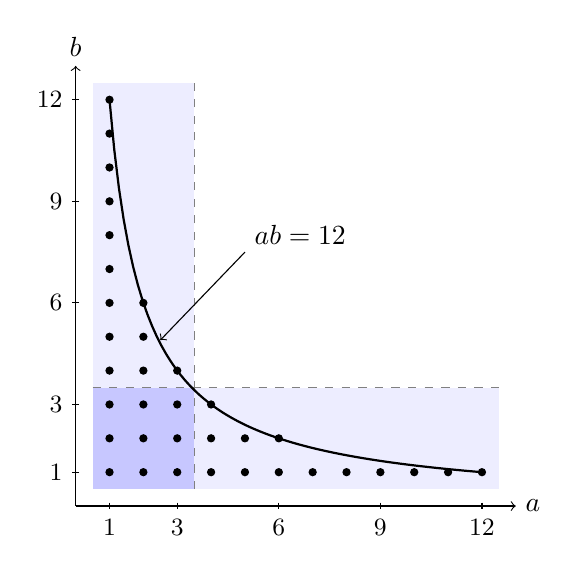
\begin{tikzpicture}[x=0.43cm,y=0.43cm]
 \fill[blue!7] (0.5,0.5) rectangle (3.5,12.5);
 \fill[blue!7] (0.5,0.5) rectangle (12.5,3.5);
 \fill[blue!22] (0.5,0.5) rectangle (3.5,3.5);
 \draw[->] (0,0) -- (13,0) node[right] {\(a\)};
 \draw[->] (0,0) -- (0,13) node[above] {\(b\)};
 \draw[dashed,gray] (3.5,0.5) -- (3.5,12.5);
 \draw[dashed,gray] (0.5,3.5) -- (12.5,3.5);
 \draw[thick,domain=1:12,samples=80] plot (\x,{12/\x});
 \foreach \a in {1,...,12} {
  \foreach \b in {1,...,12} {
   \pgfmathtruncatemacro{\within}{\a*\b<=12}
   \ifnum\within=1\relax
    \fill (\a,\b) circle (1.5pt);
   \fi
  }
 }
 \foreach \t in {1,3,6,9,12} {
  \draw (\t,0.10) -- (\t,-0.10) node[below,font=\small] {\(\t\)};
  \draw (0.10,\t) -- (-0.10,\t) node[left,font=\small] {\(\t\)};
 }
 \node[anchor=west] at (5,8) {\(ab=12\)};
 \draw[->] (5,7.5) -- (2.5,4.9);
\end{tikzpicture}
\caption{双曲线分割：圆点为 \(ab\le12\) 的正整数点。两条浅色带分别选出 \(a\le3\) 与 \(b\le3\) 的整数坐标；深色方块中的九个点需减去一次。}
\label{b3:fig:25-hyperbola}
\end{figure}

这种利用双曲线两侧对称计数的办法称为\term[dirichlet-shuangquxian-fa]{Dirichlet 双曲线法}[Dirichlet hyperbola method]。若直接把 \(\sum_{a\le x}\lfloor x/a\rfloor\) 中每项替成 \(x/a\)，会累积 \(O(x)\) 的取整误差，因而看不见线性次项。以 \(\sqrt x\) 分割以后，只需近似约 \(\sqrt x\) 项，误差便缩小到平方根尺度。若在一个很小的阈值处分割，另一方向仍会留下很长的和；平方根使两个方向的长度保持同一数量级。

部分求和还能把已有的平均值换成新的权重。由刚才的结果，置 \(c=2\gamma-1\)，可写 \(D(t)=t\log t+ct+E(t)\)，其中 \(E(t)=O(\sqrt t)\) 对所有 \(t\ge1\) 成立。取权重 \(1/n\)，得到
\begin{align*}
 \sum_{n\le x}\frac{d(n)}n
 &=\frac{D(x)}x+\int_1^x\frac{D(t)}{t^2}\,\mathrm dt\\
 &=\log x+c+\frac12(\log x)^2+c\log x+O(1)\\
 &=\frac12(\log x)^2+2\gamma\log x+O(1).
\end{align*}
这里端点的误差 \(E(x)/x=O(x^{-1/2})\) 有界，误差积分也一致有界，因为
\[
 \int_1^\infty\frac{|E(t)|}{t^2}\,\mathrm dt
 \le C\int_1^\infty t^{-3/2}\,\mathrm dt<\infty.
\]
一次计数所得的主项与误差，就这样转变成了另一个加权平均值；不需要重新逐项估计 \(d(n)\)。

\subsection{素数计数函数的应用}
\label{b3:subsec:250305}

素数的分布没有简单的逐项公式，但部分求和仍然适用。对实数 \(x\ge2\)，记
\[
 \pi(x)=\#\{p\le x:p\text{ 为素数}\},\qquad
 \vartheta(x)=\sum_{p\le x}\log p.
\]
函数 \(\pi\) 称为\term[sushu-jishu-hanshu]{素数计数函数}[prime-counting function]；函数 \(\vartheta\) 给每个素数加上对数权重。这里的 \(\pi(x)\) 是函数记号，与圆周率 \(\pi\) 应依上下文区分。

在\eqref{b3:eq:25-interval-summation}中取 \(y=2\)，令 \(a_n\) 在素数处为一、其余处为零，并取 \(f(t)=\log t\)。左端不含素数二，故
\[
 \vartheta(x)-\log2
 =\pi(x)\log x-\pi(2)\log2-\int_2^x\frac{\pi(t)}t\,\mathrm dt.
\]
因为 \(\pi(2)=1\)，两个下端项抵消，得到
\begin{equation}\label{b3:eq:25-prime-log-weight}
 \vartheta(x)=\pi(x)\log x-\int_2^x\frac{\pi(t)}t\,\mathrm dt
 \qquad(x\ge2).
\end{equation}
反过来，令 \(a_n\) 在素数处为 \(\log n\)、其余处为零，取 \(f(t)=1/\log t\)。这个权重在 \([2,x]\) 上连续可微，不涉及 \(t=1\) 的奇性。区间公式给
\[
 \pi(x)-1
 =\frac{\vartheta(x)}{\log x}-\frac{\vartheta(2)}{\log2}
       +\int_2^x\frac{\vartheta(t)}{t(\log t)^2}\,\mathrm dt.
\]
利用 \(\vartheta(2)=\log2\)，得到
\begin{equation}\label{b3:eq:25-prime-remove-weight}
 \pi(x)=\frac{\vartheta(x)}{\log x}
       +\int_2^x\frac{\vartheta(t)}{t(\log t)^2}\,\mathrm dt
 \qquad(x\ge2).
\end{equation}
两式在 \(x=2\) 时也成立，此时积分均为零。

\begin{proposition}[素数计数的两种渐近形式]\label{b3:prop:25-prime-counting-equivalence}
对实数 \(x\ge2\)，令 \(\pi(x)=\#\{p\le x:p\text{ 为素数}\}\)、\(\vartheta(x)=\sum_{p\le x}\log p\)。则当 \(x\to\infty\) 时，以下两项等价：
\[
 \vartheta(x)\sim x,\qquad \pi(x)\sim\frac{x}{\log x}.
\]
\end{proposition}
\begin{proof}
先假设 \(\vartheta(x)\sim x\)。这蕴含存在常数 \(C\)，使 \(0\le\vartheta(t)\le Ct\) 对所有 \(t\ge2\) 成立。对 \(x\ge4\)，将\eqref{b3:eq:25-prime-remove-weight}中的积分在 \(\sqrt x\) 处分开：
\begin{align*}
 0\le\int_2^x\frac{\vartheta(t)}{t(\log t)^2}\,\mathrm dt
 &\le C\int_2^{\sqrt x}\frac{\mathrm dt}{(\log t)^2}
       +C\int_{\sqrt x}^x\frac{\mathrm dt}{(\log t)^2}\\
 &\le\frac{C\sqrt x}{(\log2)^2}
       +\frac{4Cx}{(\log x)^2}
 =o\left(\frac x{\log x}\right).
\end{align*}
第一段虽不使用对数衰减，但长度只有 \(\sqrt x\)；第二段长度较大，整个区间上的对数却至少为 \(\frac12\log x\)。因此积分是低阶项，端点项 \(\vartheta(x)/\log x\sim x/\log x\) 给出所求渐近。

反过来，假设 \(\pi(x)\sim x/\log x\)。扩大常数以后，\(0\le\pi(t)\le Ct/\log t\) 对所有 \(t\ge2\) 成立。同样分割可得
\[
 0\le\int_2^x\frac{\pi(t)}t\,\mathrm dt
 \le\frac{C\sqrt x}{\log2}+\frac{2Cx}{\log x}=o(x).
\]
代入\eqref{b3:eq:25-prime-log-weight}，再用 \(\pi(x)\log x\sim x\)，便得到 \(\vartheta(x)\sim x\)。
\end{proof}

这个命题把两种计数的渐近联系起来：建立其中一种以后，Abel 求和便给出另一种。后文由 \(\zeta\) 函数的解析性质研究素数时，对数权重更自然地出现，因此会先估计带权部分和，再用这里的公式还原为素数个数。

% !TeX root = ../../Book3.tex
\section{Dirichlet 级数}
\label{b3:sec:2504}

一般幂级数以圆盘为收敛区域，Dirichlet 级数以右半平面为基本区域。原因是 \(n^{-s}=e^{-s\log n}\)，增大实部会同时压低全部高指标项。

\subsection{收敛横坐标}
\label{b3:subsec:250401}

\begin{definition}\label{b3:def:25-dirichlet-series}
形如 \(D_a(s)=\sum_{n\ge1}a(n)n^{-s}\) 的级数称为\term[dirichlet-jishu]{Dirichlet 级数}[Dirichlet series]。
\end{definition}
若级数在 \(s_0\) 收敛，令 \(b_n=a(n)n^{-s_0}\)。其尾部分和 \(\sum_{M<n\le N}b_n\) 对 \(N\ge M\) 一致趋零。对尾部应用 Abel 求和可知，对任意 \(\operatorname{Re}w>0\)，\(\sum b_nn^{-w}\) 收敛，并在 \(\operatorname{Re}w\ge\delta>0\)、\(|w|\le R\) 一致收敛。因此存在扩展实数 \(\sigma_c\)，使级数在 \(\operatorname{Re}s>\sigma_c\) 收敛且全纯，在 \(\operatorname{Re}s<\sigma_c\) 发散；边界可能随虚部而异。数 \(\sigma_c\) 称为\term[shoulian-hengzuobiao]{收敛横坐标}[abscissa of convergence]。

\subsection{绝对收敛}
\label{b3:subsec:250402}

同样定义\term[juedui-shoulian-hengzuobiao]{绝对收敛横坐标}[abscissa of absolute convergence] \(\sigma_a\)。总有 \(\sigma_c\le\sigma_a\le\sigma_c+1\)，按扩展实数理解。后一个不等式由在 \(s_0\) 收敛推出 \(a(n)n^{-s_0}\) 有界，再与 \(\sum n^{-1-\varepsilon}\) 比较得到。绝对收敛半平面的每个较小闭半平面上有统一主控，因此可以安全乘法和对素数重新分组。

\ProseParagraphBreak

对普通 \(\sum n^{-s}\)，两横坐标都为一；对交错级数，两者分别为零与一。横坐标为零的必要性可由负实部处单项不趋零看出。一个例子同时说明两横坐标可以不同，也说明一般差距上界一能达到。

\subsection{乘法}
\label{b3:subsec:250403}

\begin{proposition}\label{b3:prop:25-product-series}
若 \(D_a,D_b\) 在 \(\operatorname{Re}s=\sigma\) 都绝对收敛，则
\(D_a(s)D_b(s)=D_{a*b}(s)\) 在该直线上成立，且右侧绝对收敛。
\end{proposition}
\begin{proof}
双重绝对和为 \((\sum|a(m)|m^{-\sigma})(\sum|b(n)|n^{-\sigma})<\infty\)。因此可以按积 \(mn=r\) 分组，系数恰为有限和 \(\sum_{m\mid r}a(m)b(r/m)\)。同一个绝对和控制了右侧级数。
\end{proof}
仅仅知道两个级数逐点条件收敛，不能引用这个结论；重新分组的合法性需要另证。

\ProseParagraphBreak

在绝对收敛半平面内部还可逐项求任意次导数。设 \(\sigma_0>\sigma_a\)，再取 \(\delta>0\)。对每个固定整数 \(k\ge0\)，函数 \((\log t)^kt^{-\delta}\) 在 \(t\ge1\) 上有界。因此在 \(\operatorname{Re}s\ge\sigma_0+\delta\) 上，
\[
 \sum_n|a(n)|(\log n)^k n^{-\operatorname{Re}s}
 \le C_{k,\delta}\sum_n|a(n)|n^{-\sigma_0}<\infty.
\]
由一致收敛的导数定理，
\[
 D_a^{(k)}(s)=(-1)^k\sum_{n\ge1}a(n)(\log n)^k n^{-s}.
\]
增加对数权重会影响边界收敛，却不改变右半平面内部的全纯性。这个论证说明为什么下一节可以对 Euler 对数求导，也说明每次求导都应在离边界正距离的紧集上进行估计。

\ProseParagraphBreak

Dirichlet 级数也可视为离散测度的 Laplace 变换：将质量 \(a(n)\) 放在 \(\log n\)，则 \(n^{-s}=e^{-s\log n}\)。相应累积质量为 \(A(e^t)\)。在端点项消失的范围，变量代换 \(x=e^t\) 将部分求和写成
\[
 D_a(s)=s\int_0^\infty A(e^t)e^{-st}\,\mathrm dt.
\]
这项表示把整数上的乘法尺度变为实轴上的加法尺度。若已经知道 \(A(x)\) 的增长，积分容易估计；反过来，只知道变换在某点有极点，通常还不能恢复 \(A(x)\) 的渐近。第二十七章将增加非负性与整条边界的延拓条件，完成那个反向问题。

\subsection{系数卷积}
\label{b3:subsec:250404}

于是 \(D_d=\zeta^2\)、\(D_{\sigma_\alpha}(s)=\zeta(s)\zeta(s-\alpha)\)，最初分别在 \(\operatorname{Re}s>1\) 与 \(\operatorname{Re}s>\max(1,1+\operatorname{Re}\alpha)\) 由绝对收敛证明。\(\mathbf1*\varphi=\operatorname{id}\) 还给 \(D_\varphi(s)=\zeta(s-1)/\zeta(s)\)，但要作除法须先在此处证明分母非零，下一节的 Euler 乘积将提供这一事实。

% !TeX root = ../../Book3.tex
\section{Euler 乘积}
\label{b3:sec:2505}

算术基本定理把整数分解成素数幂，绝对收敛把这个有限分解提升为无穷乘积。对数再把乘法拆成加法，素数幂便成为自然的级数指标。

\subsection{可乘系数的 Euler 乘积}
\label{b3:subsec:250501}

\begin{theorem}[Euler 乘积]\label{b3:thm:25-euler-product}
设 \(a\) 可乘，\(\sum|a(n)|n^{-\sigma}<\infty\)。则
\[
D_a(s)=\prod_p\left(\sum_{r\ge0}a(p^r)p^{-rs}\right),\quad\operatorname{Re}s=\sigma.
\]
若 \(a\) 完全可乘，则各因子为 \((1-a(p)p^{-s})^{-1}\)。
\end{theorem}
\begin{proof}
有限多个素数的局部级数相乘，绝对收敛允许展开，所得系数正是所有仅含这些素因子的整数项。随素数集合扩大，任何固定整数最终纳入，剩余项的绝对和趋零。因此有限乘积趋于 \(D_a\)。完全可乘时局部绝对级数的收敛迫使 \(|a(p)|p^{-\sigma}<1\)，再用几何和公式。
\end{proof}
这一表示称为\term[euler-chengji]{Euler 乘积}[Euler product]。一般可乘函数的某个局部因子可能为零，故不能仅凭“有 Euler 乘积”就宣称函数无零点。几何因子情形还需证明无穷非零因子乘积不坍缩到零。

\subsection{唯一性}
\label{b3:subsec:250502}

\begin{proposition}\label{b3:prop:25-uniqueness}
两个在某个右半平面绝对收敛的 Dirichlet 级数，若代表同一函数，则对应系数相等。
\end{proposition}
\begin{proof}
对差级数，令 \(m\) 为首个非零系数指标。沿实轴 \(s=\sigma\to\infty\)，等式乘以 \(m^\sigma\) 得
\(0=a(m)+\sum_{n>m}a(n)(m/n)^\sigma\)。选绝对收敛点 \(\sigma_0\)，尾项被 \(m^{\sigma_0}|a(n)|n^{-\sigma_0}\) 控制，且逐项趋零。支配收敛得 \(a(m)=0\)，矛盾。
\end{proof}
所以解析乘法等式可以反向识别系数，但须处在确有收敛表示的公共区域。延拓后的函数值本身并不意味着原级数也在那里收敛。

\subsection{Euler 乘积的对数}
\label{b3:subsec:250503}

对 \(a(n)=1\)，\(\sum_p\sum_{r\ge1}|p^{-rs}|/r\) 在 \(\sigma>1\) 局部一致收敛，因为被常数倍的 \(\sum_p p^{-\sigma}\) 控制。于是定义
\[
L(s)=\sum_p\sum_{r\ge1}\frac{p^{-rs}}r,
\quad \zeta(s)=e^{L(s)}.
\]
等式先由有限乘积对数成立，再在局部一致极限中保持。因此 \(\zeta\ne0\) 于 \(\sigma>1\)，并且 \(L\) 是在实轴取实值的全纯对数。无零点性来自这个收敛的指数表示，不能从每个单独因子非零直接推断。

\subsection{对数导数}
\label{b3:subsec:250504}

对紧集 \(\sigma\ge1+\delta\)，导数项的绝对和
\(\sum_{p,r}(\log p)p^{-r\sigma}\) 有界：先求 \(r\) 的几何和，再与 \(\sum_{n\ge2}(\log n)n^{-1-\delta}\) 比较。因此可求导，得到
\begin{equation}\label{b3:eq:25-log-derivative}
-\frac{\zeta'(s)}{\zeta(s)}=\sum_p\sum_{r\ge1}(\log p)p^{-rs}
=\sum_{n\ge1}\frac{\Lambda(n)}{n^s},\quad\operatorname{Re}s>1.
\end{equation}
还可由有限卷积恒等式得到同一结论：\(-\zeta'(s)=D_{\log}(s)\)，而 \(\mathbf1*\Lambda=\log\)，故 \(D_\Lambda\zeta=-\zeta'\)。两条路线分别检验乘积常数与系数权重。

\subsection{对数导数中的 \texorpdfstring{\(\Lambda(n)\)}{\AnalysisPdfCapitalLambda(n)}}
\label{b3:subsec:250505}

对数本身在素数幂 \(p^r\) 处给权重 \(1/r\)；求负导数后乘上 \(r\log p\)，留下 \(\log p\)。这解释了 \(\Lambda\) 为何在所有正次素数幂处取相同值。若只保留素数一次项，所得到的不是 \(-\zeta'/\zeta\)，而会遗漏可估计但不恒零的高次幂项。

\ProseParagraphBreak

作为另一例，\(\sum\mu(n)n^{-s}=\prod_p(1-p^{-s})=1/\zeta(s)\) 在 \(\sigma>1\) 成立。它与卷积逆元 \(\mu*\mathbf1=\varepsilon\) 相符。后面若试图把这一表示向临界带推进，就必须控制 Möbius 部分和；单凭右侧已经延拓不能保证左侧条件收敛。算术抵消与解析延拓之间的区别在素数问题中尤其重要。

\begin{proposition}[平方自由整数与互素整数对的密度]
\label{b3:prop:25-two-densities}
设 \(x\ge2\)。有
\[
 \sum_{n\le x}\mu(n)^2=\frac{x}{\zeta(2)}+O(\sqrt x),
 \qquad
 \sum_{n\le x}\varphi(n)=\frac{x^2}{2\zeta(2)}+O(x\log x).
\]
其中 \(1/\zeta(2)=6/\pi^2\)。
\end{proposition}
\begin{proof}
由平方自由筛选恒等式，先交换有限和，得到
\[
 \sum_{n\le x}\mu(n)^2
 =\sum_{d\le\sqrt x}\mu(d)\left\lfloor\frac{x}{d^2}\right\rfloor
 =x\sum_{d\le\sqrt x}\frac{\mu(d)}{d^2}+O(\sqrt x).
\]
因为 \(|\mu(d)|\le1\)，把最后有限级数延到无穷的误差至多
\(x\sum_{d>\sqrt x}d^{-2}=O(\sqrt x)\)。绝对收敛的 Euler 乘积给无穷和为 \(1/\zeta(2)\)，于是得到第一式。

再令 \(N=\lfloor x\rfloor\)，计数 \(1\le a,b\le N\) 中互素的有序整数对。把 \(\sum_{d\mid\gcd(a,b)}\mu(d)\) 代入其示性函数，得
\[
 C(N)=\sum_{d\le N}\mu(d)\left\lfloor\frac Nd\right\rfloor^2.
\]
对 \(u\ge1\)，有 \(|\lfloor u\rfloor^2-u^2|\le2u\)，所以
\[
 C(N)=N^2\sum_{d\le N}\frac{\mu(d)}{d^2}
          +O\left(N\sum_{d\le N}\frac1d\right)
      =\frac{N^2}{\zeta(2)}+O(N\log N).
\]
对角线上互素的点只有 \((1,1)\)；直线 \(a=b\) 两侧由交换坐标对应。固定较大的坐标 \(n\ge2\)，其下方互素点有 \(\varphi(n)\) 个，故
\(C(N)=1+2\sum_{n=2}^N\varphi(n)=2\sum_{n=1}^N\varphi(n)-1\)。代入并把 \(N^2\) 换成 \(x^2+O(x)\)，得到第二式。\(\zeta(2)\) 的数值由前面已证的正弦乘积或相应留数计算给出。
\end{proof}

同一个常数出现在两种不同计数中，原因都可由素数局部条件解释：平方自由性要求不被 \(p^2\) 整除，互素性要求两个坐标不同时被 \(p\) 整除，两者的局部排除比例均为 \(p^{-2}\)。不过无限多个局部条件的密度不能仅凭直觉相乘。上面的有限反演、取整误差及绝对收敛尾界，才把这种解释变成有效证明。

\ProseParagraphBreak

这些平均计数不需要素数定理。它们使用 \(\sum\mu(d)/d^2\) 的绝对收敛，不要求估计 \(\sum_{d\le x}\mu(d)\) 的相消。相较之下，把 \(1/\zeta(s)\) 的 Dirichlet 级数推进到靠近实部一的边界，需要更精细的算术信息。读者应从所用权重和收敛域判断一个推导实际有多强，而不能只看公式中是否出现 Möbius 函数或素数乘积。


\begin{chaptersummary}
可乘函数由各素数幂处的数据决定；完全可乘函数进一步由各素数处的数据决定。Dirichlet 卷积在每个整数处只有有限项，因而其代数恒等式、逆元和 Möbius 反演都先于解析收敛而成立。进入级数以后，乘法需要双重绝对和，求逆需要足够靠右的收敛域，原来的有限恒等式不能替代这些条件。

Abel 求和把权重的变化与系数部分和分开，既保留抵消，也暴露端点项。它说明为何 \(A(x)=O(x^\alpha)\) 给出 \(\operatorname{Re}s>\alpha\) 的收敛，却不能自动给出边界收敛或绝对收敛。收敛横坐标描述原级数；解析延拓描述与其和函数相接的新表示，两者应始终分清。

Euler 乘积则把唯一素分解用于绝对收敛级数。完全可乘情形的对数可由可和的素数幂级数构造，随后才能安全地取对数导数与商。函数 \(-\zeta'/\zeta\) 的系数 \(\Lambda\) 记录了全部素数幂，下一章将研究 \(\zeta\) 的延拓与零点，第二十七章再把这些解析信息转回素数计数。平方自由整数及互素整数对的密度已经在本章求出，它们只依赖绝对收敛的 Möbius 权重，不需要更深的素数分布估计。
\end{chaptersummary}

\BookExercises

% 题1、3、5、8按本章已证恒等式组织为延伸应用；题2保留原d_3训练并细化误差。
% 题4、6自拟参数例，题7把正文中的发散性升级为有限截断下界。
% 公式校准：NIST DLMF 27.2（Liouville/Jordan定义）及27.4.7（Liouville级数）。
% 未据未取得全文的教材声称具体题号来源；八题均重新组织题面并给完整自证。

\begin{exercise}\label{b3:ex:25-1}
对正整数 \(n=\prod_p p^{\nu_p(n)}\)，记
\[
 \Omega(n)=\sum_p\nu_p(n),\qquad \lambda(n)=(-1)^{\Omega(n)},
 \qquad \Omega(1)=0.
\]
证明 \(\lambda\) 完全可乘，其 Dirichlet 卷积逆元为 \(\mu^2\)，并证明
\[
 \sum_{n\ge1}\frac{\lambda(n)}{n^s}
 =\frac{\zeta(2s)}{\zeta(s)},\qquad \operatorname{Re}s>1.
\]
这里 \(\mu^2(n)\) 指 \(\mu(n)^2\)，不是 \((\mu*\mu)(n)\)。
\end{exercise}
\begin{solution}
每个素数在乘积中的指数相加，故对任意正整数 \(m,n\)，
\[
 \Omega(mn)=\Omega(m)+\Omega(n),\qquad
 \lambda(mn)=\lambda(m)\lambda(n).
\]
不需要互素假设。由\cref{b3:prop:25-completely-inverse}，逆元为逐点乘积 \(\mu(n)\lambda(n)\)。若 \(n\) 含平方素因子，\(\mu(n)=0\)；若 \(n\) 为平方自由整数，则 \(\Omega(n)\) 等于不同素因子的个数，\(\lambda(n)=\mu(n)\)。包括 \(n=1\) 在内，均有 \(\mu(n)\lambda(n)=\mu(n)^2\)。

因为 \(|\lambda(n)|=1\)，其级数在 \(\operatorname{Re}s>1\) 绝对收敛。在这个范围内应用 Euler 乘积，并在各素数处使用几何恒等式，得
\[
 \sum_{n\ge1}\frac{\lambda(n)}{n^s}
 =\prod_p(1+p^{-s})^{-1}
 =\prod_p\frac{1-p^{-s}}{1-p^{-2s}}
 =\frac{\zeta(2s)}{\zeta(s)}.
\]
最后一步可先对有限乘积取商，再取极限；两个 \(\zeta\) 因子的参数实部均大于一，分母非零。此公式没有断言原级数在实部不超过一时如何收敛。
\end{solution}

\begin{exercise}\label{b3:ex:25-2}
令 \(d_3(n)\) 为满足 \(abc=n\) 的有序正整数三元组 \((a,b,c)\) 的个数。设 \(\gamma\) 为 Euler 常数，证明当实数 \(x\to\infty\) 时，
\[
 \sum_{n\le x}d_3(n)
 =\frac12x(\log x)^2+(3\gamma-1)x\log x+O(x).
\]
\end{exercise}
\begin{solution}
记 \(D(y)=\sum_{n\le y}d(n)\)。由\cref{b3:prop:25-divisor-average}，扩大误差常数后可对所有 \(y\ge1\) 写成
\[
 D(y)=y\log y+(2\gamma-1)y+O(\sqrt y).
\]
固定三元组的第一个因子 \(a\)，其余两个因子的乘积不超过 \(x/a\)，所以
\[
 \begin{aligned}
 \sum_{n\le x}d_3(n)
 &=\sum_{a\le x}D(x/a)\\
 &=x\log x\sum_{a\le x}\frac1a
   -x\sum_{a\le x}\frac{\log a}{a}
   +(2\gamma-1)x\sum_{a\le x}\frac1a
   +O\left(\sqrt x\sum_{a\le x}a^{-1/2}\right).
 \end{aligned}
\]
积分比较给 \(\sum_{a\le x}a^{-1/2}=O(\sqrt x)\)，故最后误差为 \(O(x)\)。

令 \(N=\lfloor x\rfloor\)。由调和和估计及 \(\log N=\log x+O(1/x)\)，有
\[
 \sum_{a\le x}\frac1a=\log x+\gamma+O(1/x).
\]
另一个加权和满足
\[
 \sum_{a\le x}\frac{\log a}{a}
 =\frac12(\log x)^2+O(1).
\]
为看清误差，注意 \(f(t)=\log t/t\) 在 \(t\ge e\) 上非负递减；在相邻整数区间比较 \(f\) 的上、下矩形和，离散和与积分之差被一个固定常数控制。开头有限项以及 \(N\) 到 \(x\) 的积分也有界，而 \(\int_1^x(\log t)/t\,\mathrm dt=\tfrac12(\log x)^2\)。

代入后，\(x(\log x)^2\) 的系数为 \(1-\tfrac12=\tfrac12\)；\(x\log x\) 的系数为 \(\gamma+(2\gamma-1)=3\gamma-1\)。其余项均为 \(O(x)\)，结论得证。这里三元组有序，无须除以任何排列数。
\end{solution}

\begin{exercise}\label{b3:ex:25-3}
固定整数 \(k\ge2\)，定义
\[
 J_k(n)=\#\{(a_1,\ldots,a_k)\in\{1,\ldots,n\}^k:
                 \gcd(a_1,\ldots,a_k,n)=1\}.
\]
证明
\[
 J_k(n)=n^k\prod_{p\mid n}(1-p^{-k}),\qquad
 \sum_{n\ge1}\frac{J_k(n)}{n^s}
 =\frac{\zeta(s-k)}{\zeta(s)}
 \quad(\operatorname{Re}s>k+1),
\]
并求出平均值
\[
 \sum_{n\le x}J_k(n)
 =\frac{x^{k+1}}{(k+1)\zeta(k+1)}+O_k(x^k)
 \qquad(x\to\infty).
\]
\end{exercise}
\begin{solution}
把 Möbius 约数和用于全部坐标与 \(n\) 的最大公因数。若 \(d\mid n\)，每个坐标中可被 \(d\) 整除的数有 \(n/d\) 个，因此
\[
 J_k(n)=\sum_{d\mid n}\mu(d)(n/d)^k
       =n^k\sum_{d\mid n}\frac{\mu(d)}{d^k}
       =n^k\prod_{p\mid n}(1-p^{-k}).
\]
最后一步只展开一个有限乘积，\(n=1\) 时空乘积为一。第一式也说明 \(J_k=\mu*\operatorname{id}_k\)。当 \(\operatorname{Re}s>k+1\) 时，两个因子级数绝对收敛；卷积乘法与\eqref{b3:eq:25-mobius-series}便给出所求商式。直接上界 \(J_k(n)\le n^k\) 也保证左侧绝对收敛。

为求平均值，再交换有限和：
\[
 \sum_{n\le x}J_k(n)
 =\sum_{d\le x}\mu(d)\sum_{m\le x/d}m^k.
\]
正函数 \(t^k\) 单调递增，矩形和与积分比较给出，对全部实数 \(Y\ge1\)，
\[
 \sum_{m\le Y}m^k=\frac{Y^{k+1}}{k+1}+O_k(Y^k).
\]
先在整数上以相邻上下积分夹住该和，再将 \(\lfloor Y\rfloor\) 换成 \(Y\)，所付出的误差仍为 \(O_k(Y^k)\)。于是
\[
 \sum_{n\le x}J_k(n)
 =\frac{x^{k+1}}{k+1}\sum_{d\le x}\frac{\mu(d)}{d^{k+1}}
  +O_k\left(x^k\sum_{d\le x}d^{-k}\right).
\]
由于 \(k\ge2\)，误差中的和一致有界。主项的级数延长到无穷时，误差至多为常数倍
\(x^{k+1}\sum_{d>x}d^{-k-1}=O_k(x)\)，也被 \(O_k(x^k)\) 包含。无穷和为 \(1/\zeta(k+1)\)，得到结论。若取 \(k=1\)，同一方法中的误差和成为调和和，通常只能给 \(O(x\log x)\)；这说明题目为何单列 \(k\ge2\)。
\end{solution}

\begin{exercise}\label{b3:ex:25-4}
设 \(\alpha\in\mathbb R\)，令 \(a(2^j)=2^{j\alpha}/j\)（\(j\ge1\)），其余正整数处 \(a(n)=0\)。求 Dirichlet 级数 \(D_a(s)=\sum_{n\ge1}a(n)n^{-s}\) 的两个收敛横坐标，并逐点判定边界 \(s=\alpha+\mathrm it\) 上的收敛性。
\end{exercise}
\begin{solution}
按自然顺序求和与按二的正次幂求和给出同一极限，所以
\[
 D_a(s)=\sum_{j\ge1}\frac{(2^{\alpha-s})^j}{j}.
\]
若 \(\operatorname{Re}s>\alpha\)，括号内的模小于一，级数绝对收敛；若 \(\operatorname{Re}s<\alpha\)，非零项的模为 \(2^{j(\alpha-\operatorname{Re}s)}/j\)，不趋于零。因此 \(\sigma_c=\sigma_a=\alpha\)。

在边界上，记 \(z=e^{-\mathrm it\log2}\)，于是 \(|z|=1\)。若 \(t\log2\in2\pi\mathbb Z\)，则 \(z=1\)，级数成为发散的调和级数。若 \(z\ne1\)，则
\[
 \left|\sum_{j=1}^N z^j\right|
 =\left|\frac{z(1-z^N)}{1-z}\right|
 \le\frac2{|1-z|}.
\]
以 \(1/j\) 为权重作 Abel 求和，或应用\cref{b3:prop:25-partial-sum-convergence}于指标 \(j\)，便知 \(\sum z^j/j\) 收敛。边界上的绝对级数始终为 \(\sum1/j\)，故所有非共振点均为条件收敛点。相同的两个横坐标并不能说明整条边界线的收敛行为一致。
\end{solution}

\begin{exercise}\label{b3:ex:25-5}
设 \(d(n)\) 为正整数 \(n\) 的正约数个数。证明
\[
 \sum_{n\ge1}\frac{d(n)^2}{n^s}
 =\frac{\zeta(s)^4}{\zeta(2s)},\qquad\operatorname{Re}s>1.
\]
解释为什么左侧不能直接由 \(D_d(s)^2\) 得到。
\end{exercise}
\begin{solution}
先检查绝对收敛。固定 \(\sigma=\operatorname{Re}s>1\)，在\cref{b3:prop:25-divisor-small-power}中取 \(\epsilon=(\sigma-1)/4\)，有 \(d(n)\le C_\epsilon n^\epsilon\)。故
\[
 d(n)^2n^{-\sigma}\le C_\epsilon^2 n^{-(\sigma+1)/2},
\]
右边可和。逐点平方 \(d^2\) 仍可乘，而 \(d(p^r)^2=(r+1)^2\)。

在 \(|X|<1\) 内，几何级数可逐项求导。对 \(\sum_{r\ge0}(r+1)X^r=(1-X)^{-2}\) 再施以算子 \(X\,d/dX+1\)，得到
\[
 \sum_{r\ge0}(r+1)^2X^r
 =\frac{2X}{(1-X)^3}+\frac1{(1-X)^2}
 =\frac{1+X}{(1-X)^3}
 =\frac{1-X^2}{(1-X)^4}.
\]
因此 Euler 乘积给
\[
 D_{d^2}(s)=\prod_p\frac{1-p^{-2s}}{(1-p^{-s})^4}
          =\frac{\zeta(s)^4}{\zeta(2s)}.
\]
取商时 \(\operatorname{Re}(2s)>2\)，分母确实非零。

另一方面，\(D_d^2=D_{d*d}=\zeta^4\)，其系数是四重因子计数 \(d_4\)，而非逐点平方。例如在 \(p^2\) 处，\(d(p^2)^2=9\)，但
\[
 (d*d)(p^2)=d(1)d(p^2)+d(p)d(p)+d(p^2)d(1)=10.
\]
这给出了两种乘法不同的具体检查。
\end{solution}

\begin{exercise}\label{b3:ex:25-6}
设整数 \(m\ge2\)，\(\omega=e^{2\pi\mathrm i/m}\)。求 \(\sum_{n\ge1}\omega^n n^{-s}\) 的两个收敛横坐标，并证明
\[
 \sum_{n\ge1}\frac{\omega^n}{n}
 =-\log\bigl(2\sin(\pi/m)\bigr)
   +\mathrm i\left(\frac\pi2-\frac\pi m\right).
\]
右侧的 \(\log\) 是正实数的实对数。
\end{exercise}
\begin{solution}
有限几何和给
\[
 \left|\sum_{n=1}^N\omega^n\right|\le\frac2{|1-\omega|}.
\]
部分求和遂保证实部大于零时收敛；实部不大于零时，原级数的各项模不趋于零。所以 \(\sigma_c=0\)。由于 \(|\omega^n|=1\)，绝对级数为 \(\sum n^{-\sigma}\)，故 \(\sigma_a=1\)。

为了计算边界于圆盘的幂级数值，先令 \(0\le r<1\)。在单位圆盘内积分几何级数，得
\[
 \sum_{n\ge1}\frac{(r\omega)^n}{n}=-\operatorname{Log}(1-r\omega),
\]
其中 \(\operatorname{Log}\) 取右半平面上的全纯分支，并在正实轴上等于实对数；因为
\(\operatorname{Re}(1-r\omega)>0\)，它沿此路径始终有定义。

还须证明左侧在 \(r\uparrow1\) 时趋于题目中的收敛和。对于任意尾段，\(\omega^n\) 的部分和有统一界 \(C=2/|1-\omega|\)。权重 \(r^n/n\) 对 \(n\) 非负递减，有限 Abel 求和因此给
\[
 \left|\sum_{n=N+1}^{M}\frac{r^n\omega^n}{n}\right|
 \le \frac{C}{N+1}\qquad(0\le r\le1,\ M>N).
\]
固定 \(r\) 后令 \(M\to\infty\)，此界仍成立，并且不依赖 \(r\)。先把 \(N\) 选大以控制所有尾部，再在前 \(N\) 项令 \(r\uparrow1\)，就得到所需的极限交换。

最后，
\[
 1-\omega=2\sin(\pi/m)
       \exp\left(\mathrm i\left(\frac\pi m-\frac\pi2\right)\right).
\]
这里 \(\sin(\pi/m)>0\)，辐角 \(\pi/m-\pi/2\) 落在 \((-\pi/2,0]\) 内，和已选分支一致。代入 \(-\operatorname{Log}(1-\omega)\) 即得公式。\(m=2\) 时退化为 \(\sum(-1)^n/n=-\log2\)，也核对了符号。
\end{solution}

\begin{exercise}\label{b3:ex:25-7}
证明对每个整数 \(N\ge2\)，有有限截断下界
\[
 \sum_{p\le N}\frac1p\ge\log\log(N+1)-1.
\]
证明中不得将只在 \(\operatorname{Re}s>1\) 建立的无穷 Euler 乘积直接代入 \(s=1\)。
\end{exercise}
\begin{solution}
只对有限多个素数取乘积，并把每个几何因子展开：
\[
 P_N=\prod_{p\le N}(1-p^{-1})^{-1}
 =\sum_{\substack{n\ge1\\p\mid n\Rightarrow p\le N}}\frac1n.
\]
这是有限多个绝对收敛几何级数的乘法，所以在此处没有无穷素数乘积问题。每个 \(1\le n\le N\) 的素因子都不超过 \(N\)，故
\[
 P_N\ge H_N\ge\int_1^{N+1}\frac{dt}{t}=\log(N+1).
\]
另一方面，对这个有限乘积取实对数，有
\[
 \log P_N
 =\sum_{p\le N}\frac1p
  +\sum_{p\le N}\sum_{r\ge2}\frac1{r p^r}.
\]
后面的双重和非负，且不超过
\[
 \sum_{n\ge2}\sum_{r\ge2}n^{-r}
 =\sum_{n\ge2}\frac1{n(n-1)}=1.
\]
把两边的上下界合并，得到
\(\log\log(N+1)\le\log P_N\le\sum_{p\le N}p^{-1}+1\)，即为结论。
\end{solution}

\begin{exercise}\label{b3:ex:25-8}
对整数 \(n\ge1\)，令
\[
 r_j(n)=\#\{(x_1,\ldots,x_j)\in\mathbb Z^j:
                   x_1^2+\cdots+x_j^2=n\},\qquad j=2,4.
\]
令 \(\chi_4(d)\) 在偶数处为零，在模四余一、余三处分别为一、负一，并记 \(L_4(s)=\sum_{n\ge1}\chi_4(n)n^{-s}\)。使用\cref{b3:thm:24-two-squares,b3:thm:24-four-squares}的除数公式，证明
\begin{align*}
 \sum_{n\ge1}\frac{r_2(n)}{n^s}
 &=4\zeta(s)L_4(s),&&\operatorname{Re}s>1,\\
 \sum_{n\ge1}\frac{r_4(n)}{n^s}
 &=8(1-4^{1-s})\zeta(s)\zeta(s-1),&&\operatorname{Re}s>2.
\end{align*}
再说明第二个和函数可亚纯延拓到 \(s=2\) 的一个邻域，且在那里有留数为 \(\pi^2\) 的单极点。
\end{exercise}
\begin{solution}
前章中的计数保留坐标次序和正负号，其公式为
\[
 r_2(n)=4\sum_{d\mid n}\chi_4(d),\qquad
 r_4(n)=8\sum_{\substack{d\mid n\\4\nmid d}}d.
\]
第一式即 \(r_2=4(\mathbf1*\chi_4)\)。由于 \(|\chi_4(d)|\le1\)，\(\mathbf1\) 和 \(\chi_4\) 的级数都在实部大于一时绝对收敛，卷积乘法给出第一个所求等式，并同时保证左侧绝对收敛。

对第二式，设 \(b(d)=d\) 当 \(4\nmid d\)，而 \(b(d)=0\) 当 \(4\mid d\)。于是 \(r_4=8(\mathbf1*b)\)，且在实部大于二时，
\[
 \begin{aligned}
 D_b(s)
 &=\sum_{d\ge1}d^{1-s}-\sum_{m\ge1}(4m)^{1-s}\\
 &=(1-4^{1-s})\zeta(s-1).
 \end{aligned}
\]
这些级数都绝对收敛，因此乘以 \(\zeta(s)\) 给出第二式。原计数还满足 \(r_j(0)=1\)，但题目级数从 \(n=1\) 起，零指标不能放入 \(n^{-s}\)，也没有贡献额外常数项。

由\eqref{b3:eq:25-zeta-integral}，\(\zeta(u)\) 在 \(u=1\) 附近有留数为一的单极点。因此 \(\zeta(s-1)\) 在 \(s=2\) 附近有同样的留数；\(\zeta(s)\) 在二附近则由绝对收敛级数定义为全纯函数。右侧便给出所求延拓，留数为
\[
 8(1-4^{-1})\zeta(2)=6\cdot\frac{\pi^2}{6}=\pi^2.
\]
这个数也与\cref{b3:prop:24-four-square-average}中的累计主项
\(\sum_{n\le x}r_4(n)\sim(\pi^2/2)x^2\) 相呼应：若在部分求和积分中单看主项，所得奇部为
\[
 s\int_1^\infty\frac{\pi^2}{2}t^2t^{-s-1}\,\mathrm dt
 =\frac{\pi^2s}{2(s-2)},
\]
其在二的留数正好是 \(\pi^2\)。这一比较解释常数关系；上面证明延拓和留数时，依据的是已得到的精确乘积公式。
\end{solution}
